%\textual
%[\cite{16}]
%[\citenum{1}]

\chapter{Fundamentação Teórica}

Neste capítulo são tratados os conceitos relacionados a proveniência de dados em um ambiente de computação em nuvem com a seguinte estrutura: A Seção 2.1 faz uma pequena revisão da definição e de modelos de proveniência. A Seção 2.2 mostra as alternativas de bancos de dados utilizados na computação em nuvem. E por último a Seção 2.3 apresenta alguns trabalhos presente na literatura sobre proveniência de dados.

\section{Proveniência de Dados}

O termo Proveniência de dados diz respeito à origem ou procedência dos dados. A proveniência também estar relacionada à auditoria, triagem, linhagem e origem do dado \cite{davidson}. A proveniência ajuda a responder questões sobre os dados, tais como: quem criou este dado e quando, quando o dado foi modificado e por quem e qual foi o processo usado para criar o dado.

De acordo com \cite{davidson}, a proveniência pode ser dividida em três tipos:
\begin{itemize}
\item Prospectiva: trata-se da sequência de processos utilizados (receita) para a geração do dado, ou seja, captura os passos que devem ser seguidos para a geração de um dado produto.
\item Retrospectiva: trata-se das informações obtidas durante a execução dos processos de geração do dado. Compreende desde o tempo de duração de cada atividade executada até a origem dos dados de entrada. Além disso, não depende do tratamento da proveniência prospectiva para ser utilizado. Em outras palavras, é como se fosse um \textit{log} detalhado da execução de uma tarefa.
\item Dados definidos pelo usuário: qualquer informação que o usuário julgar necessária para futura utilização. Como exemplo, pode-se citar anotações, conclusões a respeito do processo e, até mesmo, observações sobre parâmetros utilizados.
\end{itemize}

Segundo \cite{tan}, a obtenção da proveniência pode seguir duas abordagens, abordagem preguiçosa (\textit{lazy}) na qual a obtenção da proveniência é executada somente no momento que é solicitada, e abordagem ansiosa (\textit{eager}) na qual a proveniência é obtida durante a geração da informação e é armazenada para permitir futuras consultas. Cabe ressaltar que as duas abordagens podem ser combinadas, fazendo com que algumas informações sejam obtidas pela abordagem preguiçosa e outras pela ansiosa.

Ainda segundo \cite{davidson}, quando a proveniência é capturada de forma automática, pode-se dividir o nível em que é feita a captura conforme segue:
\begin{itemize}
\item \textit{Workflow}: envolve a descrição da execução de um processo, ou seja,  das tarefas que dele fazem parte, é usado pela grande maioria das soluções com SGWfC (Sistemas de Gerência de \textit{Workfow} ) e nesse caso deve ser adaptado para capturar os dados dos diferentes processos executados;
\item Atividade: pode ocorrer de duas formas. Na primeira, cada processo executado é alterado para capturar os dados de proveniência. Na segunda, podem ser criados programas específicos para monitorar a execução de um determinado processo e capturar os dados de proveniência;
\item Sistema Operacional: utiliza os dados fornecidos pelo próprio sistema operacional como insumo para a proveniência.
\end{itemize}

Modelos de proveniência de dados tem como principal objetivo fornecer uma estrutura para que os dados de proveniência possam ser armazenados e recuperados, mantendo seu significado e potencializando os seus benefícios. Para modelar os dados de proveniência foram especificados alguns modelos, tais como:

\begin{itemize}
\item \textit{W7}: foi apresentado por \cite{ram} e tem como base a ontologia de Bunge \cite{bunge}, a qual objetiva descrever as propriedades de um objeto de caráter geral. A partir deste estudo, o modelo \textit{W7} estruturou a proveniênica de uma peça de dado através da resposta a 7 perguntas (ou dimensões): O que?, Quem?, Quando?, Onde?, Como?, Qual?, e Por quê?.
\item \textit{Provenance Vocabulary}: descrito por \cite{zhao} volta sua atenção para o problema da proveniência de dados publicados na web. A sua principal característica é fornecer classes e propriedades para que publicadores de dados para \textit{web} possam armazenar, além dos dados publicados, também os metadados com informações úteis sobre a proveniência dos dados publicados.
\item \textit{Provenir Ontology}: descrito por \cite{sahoo} foi desenvolvido para ser um modelo de proveniência de dados genético, priorizando a interoperabilidade entre diferentes sistemas e sua adaptação para qualquer aplicação. Da mesma forma que no modelo \textit{Provenance Vocabulary}, o modelo \textit{Provenir Ontology} define um núcleo comum e permite a criação de módulos específicos para o domínio da aplicação desejada.
\item OPM (\textit{Open Provenance Model}): começou a ser discutido em maio de 2006 no \textit{Workshop} Internacional de Anotação e Proveniência. É um modelo aberto voltado a caracterização da proveniência de qualquer "coisa'', material ou imaterial. O modelo OPM, descrito em \cite{moreau} procura demonstrar a relação causal entre eventos que afetam objetos (digitais ou não) e descreve essa relação através de um grafo acíclico direcionado.
\end{itemize}

\subsection{PROV-DM - Provenance Data Model}

O PROV-DM teve a sua primeira versão desenvolvida em outubro de 2011 sendo uma recomendação do W3C. A sua versão mais nova foi publicada em abril de 2013. Este modelo tem como principal função descrever as pessoas, entidades e atividades envolvidas na produção de uma peça de dado ou de um objeto qualquer. Sendo assim, o modelo cria as condições para que a proveniência seja demonstrada e trocada entre diferentes sistemas.
O modelo PROV-DM tem como principal característica demonstrar a proveniência de qualquer objeto (real ou imaginário) através de um grafo direcionado. A raiz deste grafo representa a entidade cuja proveniência está sendo representada e as arestas são direcionadas para as atividades e entidades das quais foram originadas.

O modelo é dividido em seis componentes que contém tanto os elementos como as relações possíveis entre eles \cite{w3c}.

\begin{itemize}
\item Entidades: entidades (\textit{Entities}) podem representar qualquer objeto (real ou imaginário); 
\item Atividades: atividades (\textit{Activities}) é algo que ocorre ao longo de um período de tempo e atua sobre ou com entidades;
\item Agente e responsabilidades: Agentes (\textit{Agents}) são entidades que influenciam, direta ou indiretamente, a execução das atividades, recebem atribuições de outros agentes e podem ter algum tipo de ligação (posse, direitos, etc...) sobre outras entidades;
\item Derivações: descreve a relação entre diferentes entidades durante o ciclo de transformação executado pelas atividades permitindo demonstrar a dependência entre as entidades usadas e geradas;
\item Coleções: são Entidades que possuem membros, os quais são também entidades, e podem ter a sua proveniência demonstrada de forma coletiva;
\item Anotações: fornece mecanismos para inclusão de anotações para os elementos do modelo.
\item Plano: Representa um conjunto de ações ou passos que um Agente deve seguir para chegar a um determinado objetivo
\item Conta: Representa um conjunto de informações (tipos e relações) que compõe um grafo de proveniência.
\end{itemize}

A Figura \ref{fig:entidadeprovdm} ilustra os símbolos utilizados pelo modelo PROV-DM para representar os diferentes nós do grafo. O símbolo da Entidade também é utilizado para representar os tipos Coleção e Plano, uma vez que representam subtipos do tipo Entidade. O tipo Conta não tem símbolo pois representa o próprio grafo de proveniência.

\begin{figure}[!ht]
\centering
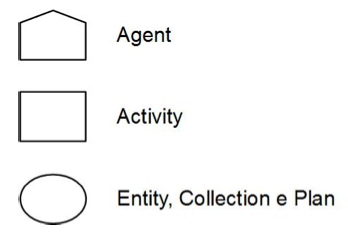
\includegraphics[width=230pt]{images/Figura21.png}
\caption{Representação gráfica dos diferentes tipos no modelo PROV-DM \cite{w3c}.}
\label{fig:entidadeprovdm}
\end{figure}

As relações representam as arestas no grafo de proveniência que, por sua vez, indicam as relações possíveis entre cada nó. Além de descrever cada tipo que compõe o modelo, os seis componentes também detalham as relações que podem ocorrer entre cada um dos tipos. A seguir são descritas as algumas relações:

\begin{itemize}
\item \textit{wasDerivedFrom}: indica, de forma geral, que uma Entidade (original) foi usada, direta ou indiretamente, na geração de outra Entidade (derivada);
\item \textit{used}: indica que uma Entidade foi usada por uma Atividade;
\item \textit{wasGeneratedBy}: indica que uma Entidade foi gerada por uma Atividade;
\item \textit{wasAttributedTo}: atribui algum tipo de responsabilidade a um Agente sobre uma Entidade;
\item \textit{wasAssociatedWith}: atribui algum tipo de responsabilidade a um Agente sobre uma Atividade;
\item \textit{actedOnBehalfOf}: indica que um Agente está agindo em nome de outro.
\end{itemize}

A fim de permitir um histórico mais detalhado das derivações feitas durante o processo representado pela proveniência, a relação \textit{wasDerivedFrom} possui diversos subtipos.

A seguir tem-se a descrição dos subtipos da relação \textit{wasDerivedFrom} \cite{w3c}:

\begin{itemize}
\item \textit{wasQuotedFrom}: indica que a Entidade derivada foi gerada a partir da cópia de parte da Entidade original;
\item \textit{hadOriginalSource}: indica que uma Entidade corresponde a fonte da informação que corresponde a Entidade derivada;
\item \textit{wasRevisionOf}: indica que a Entidade derivada foi gerada a partir da revisão da Entidade derivada, sendo que tal responsabilidade da revisão pode ser atribuída a um Agente;
\item \textit{tracedTo}: indica, de forma genérica, que existe uma relação de dependência entre duas Entidade, sem especificar qual é a derivada nem qual é a original.
\end{itemize}

O tipo de restrição mais importante é chamada restrição de ordem dos eventos. Neste tipo de restrição se pressupoem que os elementos do grafo de proveniência são dotados de características temporais representadas por propriedades como hora inicial ou final e que podem ser avaliadas e validadas. Tal validação pretende garantir que um grafo de proveniência represente uma ordem de acontecimentos possíveis.

As restrições são dividias em três grupos: restrições de Atividade, restrições de Entidade e restrições de Agente.  A seguir são descritas as restrições relevantes para este trabalho:

\begin{itemize}
\item Restrições de Atividade - restrições relacionadas à execução das Atividades. Exemplos:
  \begin{itemize}
    \item Início/Fim - o início da execução de uma Atividade deve preceder o seu fim;
    \item Uso: o uso de uma Entidade por uma Atividade deve ocorrer entre o início e o fim da sua execução;
     \item Geração - a geração de uma Entidade por uma Atividade deve ocorrer entre o início e o fim da sua execução.
  \end{itemize}
\item Restrições de Entidade - restrições relacionadas ao ciclo de vida de uma Entidade. Exemplos:
  \begin{itemize}
    \item Geração/Uso: a geração de uma Entidade deve preceder o seu uso;
    \item Derivação/Uso/Geração: para os casos em que existe uma derivação entre duas Entidades, por exemplo E2 é derivado de E1, e o uso de E1 é conhecido, então o uso de E1 deve preceder a geração de E2;
    \item Derivação/Geração/Geração: para os casos em que existe uma derivação entre duas Entidades, por exemplo E2 é derivado de E1, e o uso de E1 não é conhecido, então a geracção de E1 deve preceder a geração de E2.
  \end{itemize}
\item Restrições de Agente - restrição relacionada ao ciclo de vida de um Agente:
  \begin{itemize}
    \item Associação: a associação entre um Agente e uma Atividade deve ocorrer entre o início e o fim da execução desta Atividade.
  \end{itemize}
\end{itemize}

O modelo PROV-DM fornece um recurso para adição de informações extras no grafo de proveniência através de um identificador chamado Nota (\textit{Note}). Este identificador representa um conjunto de pares atributo-valor que permite ao usuário criar diversos tipos de anotações. Cada Nota, por sua vez, pode ser conectada a qualquer tipo ou relação existente no grafo a partir de uma relação chamada \textit{hasAnnotaion}. A Figura \ref{fig:grafoproveniencia} mostra um exemplo de grafo baseado no modelo PROV-DM. Na figura podem ser vistas quatro anotações, sendo duas relacionadas às arestas \textit{wasAssocitedWith} informando o papel de cada Agente na Atividade, uma relacionada com a Atividade e outra relacionada com a Entidade gerada.

\begin{figure}[h!]
\centering
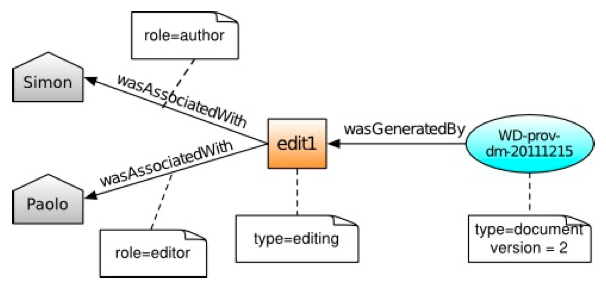
\includegraphics[width=300pt]{images/grafoproveniencia.png}
\caption{Exemplo de grafo do modelo PROV-DM que utiliza Nota \cite{w3c}.}
\label{fig:grafoproveniencia}
\end{figure}

A escolha do PROV-DM deu-se baseada em \cite{renato} onde é apresentada uma comparação entre os principais modelos de proveniência de dados disponíveis na literatura. Os principais requisitos considerados foram:
\begin{itemize}
\item Capacidade de representar a proveniência de uma peça de dado, descrevendo os processos e insumos utilizados em sua geração;
\item Uma representação gráfica adequada, com diferentes símbolos para cada elemento, e relações suficientes para demonstrar a proveniência de forma objetiva;
\item Símbolo para representar grandes conjuntos de dados;
\item Extenso material disponível cobrindo diferentes aspectos da proveniência de dados;
\item O fato de estar sendo desenvolvido pelo W3C e vindo a ser recomendação desta instituição em 2013;
\item Capacidade do modelo de proporcionar o intercâmbio de informações entre diferentes sistemas.
\end{itemize}

Dessa forma, de acordo com \cite{renato} a aplicação do modelo PROV-DM para representar a proveniência de dados em projetos de bioinformática, se mostrou bastante simples e direta. Os componentes do modelo, tais como o agente, atividade e coleção, representam elementos presentes em grande parte dos experimentos executados em projetos de bioinformática. As relações, por sua vez, demonstram de forma objetiva as dependências entre cada elemento no grafo, e a utilização das regras e do tipo de derivação permitem maior grau de especificidade quando necessário.

\section{Armazenamento de Dados na Nuvem baseado em NoSQL}

O modelo de computação em nuvem foi desenvolvido com o objetivo de fornecer serviços de fácil acesso e de baixo custo, garantindo três benefícios. O primeiro benefício é reduzir o custo na aquisição e composição de toda infraestrutura necessária para atender as empresas. O segundo é a flexibilidade que esse modelo oferece no que diz respeito à adição e troca de recursos computacionais, podendo escalar tanto em nível de \textit{software} como em nível de \textit{hardware}. O último benefício é prover uma abstração e facilidade de acesso aos usuários destes serviços.

Infraestruturas, plataformas e \textit{software} estão sendo disponibilizados como serviços, sendo estes fornecidos por ambientes de Computação em Nuvem, no qual empresas e usuários podem alugar capacidade de computação e armazenamento de forma transparente e sob demanda. Estas empresas e usuários estão movendo seus dados e aplicações para a nuvem de forma a acessá-los a qualquer momento e independente de localização. Entretanto, este novo modelo de computação requer grandes mudanças nos sistemas de gerenciamento de dados, pois estes sistemas necessitam de escalabilidade, disponibilidade, desempenho e custo \cite{sousa}.

Com a popularização da internet e o aumento na geração de dados, o volume se torna um grande desafio para os bancos de dados relacionais convencionais que se mostraram ineficientes, uma vez que não possuem escabilidade quando existe uma grande quantidade de dados armazenados. Dessa forma, aspectos de armazenamento de dados, processamento de consultas e controle transacional têm sido flexibilizados por algumas abordagens para garantir a escabilidade, mas ainda não existem propostas na literatura que combinem estes aspectos de forma a melhorar o desempenho sem comprometer a consistência dos dados \cite{sousa}.

Surgiram alguns sistemas não-relacionais que gerenciam grandes volumes de dados e, em geral, fornecem garantias de consistência fraca, estruturas e interfaces simples, que foram classificados como bancos \textit{NoSQL} (\textit{Not Only SQL}).

Os bancos \textit{NoSQL} podem ser classificados em quatro classes gerais \cite{rabi}:

\begin{itemize}
\item Chave/Valor: os dados são armazenados como pares chave-valor que são indexados para recuperação por chaves.  Os mais populares são o \textit{Riak} \cite{riak}, \textit{Redis} \cite{redis}, \textit{Memcached}, \textit{Berkeley DB} \cite{berkeley}, \textit{Amazon DynamoDB} \cite{dynamodb}, \textit{Porject Voldemort} \cite{pvoldemort} e \textit{HamsterDB} \cite{hamsterdb}.
\item Orientado a coluna: armazena os dados em linhas com colunas associadas, fazendo uso de uma chave de linha. Famílias de colunas são grupos de dados relacionados que, frequentemente, são acessados juntos \cite{fowler}. Exemplos são o \textit{BigTable} \cite{chang2008bigtable}, \textit{Cassandra} \cite{cassandra} e \textit{HBase} \cite{hbase}.
\item Armazenamento baseado em documentos: os dados são armazenados e organizados como uma coleção de documentos. Eles armazenam documentos baseados no formato \textit{JSon}, XML, BSON, entre outros. Exemplos são o \textit{MongoDB} \cite{mongodb}, \textit{Apache CouchDB} \cite{couchdb} e \textit{RavenDB} \cite{ravendb}.
\item Bancos de dados de grafos: atividades sobre bancos de dados de grafos surgiram na primeira metade dos anos noventa e depois desapareceram. Resurgindo recentemente devido a projetos onde este estilo de base de dados é necessário (por exemplo química, biologia, mineração e semântica web)\cite{angles}. Eles permitem armazenar entidades e também relacionamentos entre essas entidades. Entidades também são conhecidas como nodos, os quais possuem propriedade. Os relacionamentos são conhecidos como arestas que podem ter propriedades. Exemplos são \textit{Neo4J} \cite{neo4j}, \textit{Infinite Graph} \cite{infinitegraph} ou \textit{FlockDB} \cite{flockDB}.
\end{itemize}

\subsection{Modelo de Dados de Grafo}

Os bancos de dados relacionais tem sido a principal solução adotada pela indústria por décadas, porém muitas aplicações estão buscando modelos de dados alternativos, devido a ineficiência do modelo relacional quando se precisa realizar muitas junções com tabelas grandes. 

Um outro desafio é o armazenamento de dados em aplicações que tem colaboração interativa e compartilhamento de informações, tais como \textit{Facebook}, \textit{Linkedln} e \textit{Flickr}. Outras aplicações onde bancos de dados de grafos podem ser aplicados é a interação genética, onde nós representam proteínas, e as arestas entre os nós representam as interações físicas entre proteínas. Aplicações que envolvem a análise de redes para sistemas de recomendação, com o objetivo de apresentar informações que possam ser interessantes para os usuários com base em conhecimento prévio extraído do ambiente social.

O  modelo de dados de grafo é uma estrutura na qual o esquema e/ou instâncias são modeladas como um grafo dirigido, possivelmente rotulado, ou generalizações da estrutura de dados do grafo, onde a manipulação de dados é expressa por operações orientadadas para o grafo e construtores de tipos, e restrições de integridade que podem ser definidas sobre a estrutura do grafo \cite{angels}.

Normalmente, os bancos de dados de grafos são aplicados onde a informação sobre a interconectividade entre os dados ou topologia é mais importante, ou tão importante, quanto os dados. Tem-se em \cite{angels} as principais vantagens de se usar esse tipo de modelo:

\begin{itemize}
\item Permite uma modelagem mais natural dos dados porque as estruturas de grafos são visíveis para o usuário.
\item Permite expressar as consultas em um nível maior de abstração.
\item Permite a implementação de algoritmos eficientes para realizar específicas operações.
\end{itemize}

A representação de entidades e relações é fundamental para os modelos de grafos. Uma entidade ou objeto representa algo que existe como uma unidade simples e completa. Uma relação é uma propriedade ou predicado que estabelece uma conexão entre duas ou mais entidades. No entanto, dependendo da aplicação em particular, o modelo grafo pode ser diferente, mostrando um grau de complexidade diferente.

Em \cite{dominguez}, tem-se uma descrição de alguns componentes importantes como:

\begin{itemize}
\item Atributos: além de nós e arestas, bancos de dados de grafos armazenam informações associadas a esses nós e arestas. A informação é tipicamente uma \textit{string} ou valores numéricos, que indicam as características da entidade ou relação. Para o caso particular de arestas, alguns grafos incluem atributos numéricos que quantificam a relação, na qual é geralmente interpretada como o comprimento, peso, custo ou a intensidade da relação. Além disso, muitas aplicações podem definir um identificador exclusivo para cada nó e aresta do grafo com o objetivo de rotular cada elemento gráfico;
\item Direcionamento: dependendo do problema a relação entre dois nós pode ser simétrica ou não. Se a relação é simétrica, as duas pontas da aresta são diferentes, mas indistinguíveis, ou seja, não há ponta inicial nem ponta final. Se a relação não é simétrica, é possível diferenciar as duas pontas da aresta, em outras palavras, a ponta inicial da aresta é o nó a partir do qual começa a aresta, e a ponta final da aresta é o nó na qual a aresta termina;
\item Nós e arestas rotuladas: em algumas aplicações, é possível diferenciar rótulos (ou tipos) de nós e arestas. Rotulagem tem um impacto importante porque alguns aplicativos requerem distinção entre os diferentes tipos de relações. Por exemplo, uma rede social pode aceitar relações ''positivas'' ou ''negativas'' de amizade;
\item Multigrafos: diferem dos grafos em que dois nós podem ser conectados por várias arestas. Multigrafos aparecem geralmente quando grafos possuem arestas diferenciadas porque muitas vezes dois nós estão relacionados por diferentes categorias. Por exemplo, em uma rede de telefonia móvel, que representa os telefones celulares como os nós e ligações telefônicas como as arestas, dois nós terão múltiplas conexões;
\item Hipergrafos: um hipergrafo é uma generalização do conceito de um grafo, no qual as arestas são substituídos por hiperarestas. Uma hiperaresta liga um número arbitrário de nós. Hipergrafos são utilizados, por exemplo, para a construção de modelos de inteligência artificial.
\end{itemize}

Ainda, de acordo com \cite{dominguez}, há vários tipos de operações importantes em grafos. Essas operações não são típicas de um domínio específico, mas são operações que podem ser necessárias em algum contexto. As principais operações são:

\begin{itemize}
\item Travessias: são operações que se iniciam de um único nó e explora recursivamente os vizinhos até que uma condição final, tais como a profundidade ou visitar um nó de destino seja alcançado;
\item Análise Gráfica: basicamente inclui o estudo da topologia de grafos para analisar a sua complexidade e para caracterizar objetos do grafo. É basicamente usado para verificar algumas distribuições de dados específicos, para avaliar um padrão específico, ou para obter informações detalhadas sobre o papel de nós e arestas;
\item Componentes: um componente conectado é um subconjunto de nós do grafo onde existe um caminho entre qualquer par de nós. Assim, apenas um nó pertence a um único componente conectado do grafo. Encontrar componentes conectados geralmente é crucial em muitas operações, normalmente utilizados em uma fase de pré-processamento. Além disso, algumas operações são úteis para estudar a vulnerabilidade de um grafo, ou a probabilidade de separar um componente conectado em dois outros componentes;
\item Comunidades: é geralmente considerada como um conjunto de nós, onde cada nó é mais próximo dos nós dentro da comunidade do que dos nós fora dela;
\item A correspondência de padrões: reconhecimento de padrões lida com algoritmos que visam reconhecer ou descrever padrões de entrada. Padrões de grafos são geralmente classificados em exato ou aproximado;
\item Equivalência estrutural: encontrar semelhança entre nós em um grafo tem se mostrado muito importante em problemas de análise de redes socias, ou seja, refere-se à medida em que nós têm um conjunto de ligações com outros nós do sistema;
\item Transformação: compreende as operações que alteram o banco de dados de grafo: cargas de um grafo, adicionar/remover nós ou arestas dos grafos, criar novos tipos de nós/arestas/ atributos ou modificar o valor de um atributo. O resto das consultas são consideradas consultas de análise;
\item Acesso em cascata: uma operação segue um padrão em cascata se a consulta executa operações com uma profundidade de pelo menos dois nós. Já uma operação que não seja em cascata pode acessar apenas um nó, uma aresta ou vizinhos de um nó;
\item Escala: classificam-se as consultas, dependendo do número de nós acessados. Pode-se distinguir dois tipos de consultas, consultas globais e de proximidade. Em outras palavras, considera-se como consultas globais aquelas que acessam todos os nós ou as arestas do grafo, já as de proximidade acessam apenas uma parte do gráfico;
\item Atributos: bancos de dados não só tem que gerir a informação estrutural do grafo, mas também dos dados associados às entidades do grafo. Aqui, classificam-se as consultas de acordo com o conjunto de atributos que ela acessa: conjunto de atributos da aresta, atributos do nó, atributos do nó e da aresta ou sem atributos;
\item Resultado: diferenciam-se três tipos de resultados: grafos, agregados e conjuntos. A saída mais comum para uma consulta de banco de dados grafo é outro grafo, que é normalmente uma transformação, uma seleção ou uma projeção do grafo original, que inclui nós e arestas. O segundo tipo de resultados é a construção de agregados, cuja aplicação mais comum é resumir as propriedades do grafo. Finalmente, um conjunto é uma saída que contém tanto as entidades atômicas ou conjuntos de resultados que não estão organizados na forma de grafos.
\end{itemize}

Há uma grande variedade de modelos de bancos de dados de grafos, sendo que cada modelo de grafo é otimizado para um conjunto específico de funcionalidades ou consultas. Segundo \cite{buerli}, os bancos de dados de grafos podem ser classificados em:
\begin{itemize}
\item Bases de dados de grafos: fornecem um modelo tradicional de objetos para nós e relacionamentos.
\item Bases de dados de grafos distribuídas: abstrai a distribuição de grandes grafos.
\item Bases de dados de grafos baseados em chave-valor: simplificam o modelo de objetos relacionados aos bancos de dados de grafos para permitir uma maior escalabilidade horizontal. Esses modelos são contruídos sobre um banco de chave-valor existente.
\item Bases de dados de grafos baseados em documentos: adiciona a complexidade de bancos de dados baseados em documentos a um nó de uma base de dados de grafo.
\item Bases de dados de grafos baseados em SQL: a estrutura de um grafo é criado sobre um banco de dados SQL.
\item Bases de dados de grafos baseados em \textit{Map-Reduce}: permite a manipulação de grandes grafos, tem o objetivo de aumentar ao máximo o paralelismo, particionando os nós do grafos entre diversas máquinas.
\end{itemize}

\subsection{Banco de dados relacional versus Banco de dados de grafo}

Um estudo feito por \cite{chad} compara uma base de dados relacional, como MySQL, com o modelo de grafos, tal como \textit{Neo4J}, para armazenamento de dados de proveniência. Ele propõe um \textit{benchmark} objetivo e uma comparação subjetiva baseada na documentação e experiência. Os testes objetivos incluem a velocidade de processamento em um conjunto de consultas pré-definidas, requisitos de espaço em disco e escabilidade. Já, os testes subjetivos incluem maturidade/nível de suporte, facilidade de programação, flexibilidade e segurança.

A comparação objetiva mostrou que os bancos de dados de grafos apresentaram melhor desempenho do que os bancos de dados relacionais em consultas estruturais e que envolvem busca de textos. Entretanto, devido ao fato do mecanismo de indexação usado em bancos de grafos ser baseado em \textit{strings}, as consultas que envolvem contagem numérica apresentaram menor eficiência.

Já a comparação subjetiva mostrou que em relação ao nível de maturidade/suporte os bancos de dados de grafos, em geral, possuem um mercado menor, consequentemente menos usuários, ausência de uma linguagem unificada e suporte. Em relação à facilidade de programação, depende do problema, para consultas transversais no grafo é mais simples em bancos de dados de grafos enquanto procurar valores de atributos em uma tabela é extremamente fácil com o modelo relacional.

Quanto a flexibilidade o modelo de grafos, especificamente o \textit{Neo4J}, tem um esqema facilmente mutável. O esquema do modelo relacional pode ser alterado, porém fazer isso é mais complexo do que no modelo de grafos. E por fim, quanto a segurança, o modelo relacional possui suporte interno a multi-usuários, por outro lado, muitas bases de dados de grafos não possuem suporte para ambientes multi-usuários. Portanto, de acordo com \cite{chad}, o modelo de dados de grafos ainda se apresenta prematuro para ser executado em um ambiente de produção.

Em seu livro \textit{Neo4J In Action}, \cite{partner2013neo4j} executou um experimento comparando um banco de dados relacional com o banco de dados de grafos \textit{Neo4J}. O experimento consite em encontrar amigos de amigos em uma rede social com uma profundidade de no máximo 5 nós, ou seja, dada duas pessoas escolhidas aleatoriamente, há um caminho que as conecta com no máximo 5 relações? A base de dados foi populada com um 1.000.000 de pessoas, sendo que cada uma com aproximadamente 50 amigos.

Conforme mostra a Tabela \ref{tab:mysqlneo4j}, em uma profundidade de dois nós (amigos de amigos), ambos os modelos de dados apresentam uma boa performance. Já com uma profundidade de 3 nós (amigo de amigo de amigo) os bancos de dados de grafos conseguem reduzir o tempo de execução da consulta consideravelmente. E finalmente, para encontrar todos os amigos até uma profundidade de cinco nós, os bancos de dados relacionais simplesmente não conseguiram finalizar a consulta, enquanto o \textit{Neo4J} retorna o resultado em aproximadamente dois segundos.

\begin{table}[!h]
\centering
  \large
  \setlength{\arrayrulewidth}{2\arrayrulewidth}
  \setlength{\belowcaptionskip}{10pt}
  \caption{\ Comparação MySQL versus Neo4J. \cite{partner2013neo4j}}
  \scalebox{0.8}{
\begin{tabular}{|c|c|c|c|}
\hline
\multicolumn{1}{|l}{Profundidade} & 
\multicolumn{1}{|l}{\begin{tabular}[c]{@{}c@{}}Tempo de execução\\  no MySQL (s)\end{tabular}} &
\multicolumn{1}{|l}{\begin{tabular}[c]{@{}c@{}}Tempo de execução\\  no Neo4J (s)\end{tabular}} &
\multicolumn{1}{|l|}{Registros retornados} \\ \hline
2                                 & 0.016                                                                                          & 0.01                                                & 2.500                                      \\ \hline
3                                 & 30.267                                                                                         & 0.168                                               & 110.000                                    \\ \hline
4                                 & 1543.505                                                                                       & 1.359                                               & 600.000                                    \\ \hline
5                                 & ---                                                                                            & 2.132                                               & 800.000                                    \\ \hline
\end{tabular}}
\label{tab:mysqlneo4j}
\end{table}


\section{Trabalhos Relacionados}

A seguir são apresentados alguns trabalhos relacionados a proveniência de dados que focam no modelo de proveniência usado, ambiente de execução no qual a proveniênca é capturada e sistema de armazenamento de dados utilizado.

Pode-se ver a importância da proveniência em ambientes de computação em nuvem em \cite{kiran}, que  defende a proveniência como primeiro conjunto de dados a ser salvo trazendo benefícios tanto para os provedores de armazenamento (como \textit{Amazon}) como para os usuários. Os provedores de armazenamento em ambiente de computação em nuvem podem tirar proveito das informações inerentes a proveniência de dados para diversas aplicações que vão desde a aplicações de segurança, pesquisa a melhoria de desempenho. Por sua vez, os usuários reduzem esforço de desenvolvimento extra para o armazenamento da proveniência.

Em \cite{muniswamy} trata sobre os benefícios de realizar proveniência na computação em nuvem, principalmente em projetos científicos, que é importante para o usuário saber informações como \textit{cluster}, nodos, bancos usados, parâmetros de entrada e saída, tempo de execução, métodos invocados e processos iniciados e finalizados, porque há a necessidade de reproduzir o experimento, ajustar os parâmetros de entrada do \textit{workflow} e comparar os resultados. Tudo isso com o objetivo de obter a validação do projeto.

Em \cite{paulino}, tem-se uma abordagem que apoia a coleta de metadados de proveniência em experimentos científicos, baseada na evolução da arquitetura \textit{Matrioska} para o ambiente de nuvens. Além disso, também apresenta um modelo de dados capaz de armazenar os metadados de proveniência específicos da nuvem baseado no modelo \textit{Open Provenance Model}. Para validação do trabalho foi aplicado como estudo de caso um \textit{workflow} de Mineração de Texto (MT) concebido e executado com o SGWfC (Sistema de Gerência de \textit{Workflow}) \textit{Vistrails} e como resultado conseguiu-se capturar um conjunto inicial de dados que não podiam ser coletados somente com os mecanismos locais de proveniência dos SGWfC, tais como, os identificadores de produtos de dados e a identificação das instâncias utilizadas (endereço IP), instância e o tipo de banco de dados e quais usuários executaram o \textit{workflow}.

Uma abordagem desenvolvida na forma de um componente de software chamada \textit{ReproeScience} para reprodução do ambiente onde o experimento computacional foi originalmente executado, de forma que o mesmo possa ser instanciado sob demanda e reproduzido em iguais condições foi proposto por \cite{oliveira}. O \textit{software} desenvolvido usa um modelo de dados baseados no modelo de proveniência PROV-DM. O \textit{ReproeScience} coleta dados de proveniência por meio de sinais do sistema operacional, tais como interrupções e \textit{system calls}, em seguida executa uma atividade de clonagem do ambiente original gerando imagens de máquinas virtuais prontas para serem reproduzidas em uma estação de trabalho ou na nuvem.

Devido a grande quantidade de dados gerados durante um experimento científico, pode ser inviável analisar os dados após a execução. Por isso, \cite{costa} propõe uma solução para monitorar o experimento durante a sua execução usando dados de proveniência que podem ser capturados tanto em ambientes \textit{dekstop} como de computação em nuvem. A análise da proveniência em tempo de execução permitirá aos cientistas monitorar o \textit{workflow} e tomar ações antes do seu final. O modelo de proveniência PROV-DM foi usado como base para a geração da modelagem do banco de dados. Para a captura foram desenvolvidos diversos componentes que executam em paralelo com o \textit{workflow} e importam os dados gerados pelos diferentes SGWfC para a base de dados PROV-Wf. Uma vez todas as informações de proveniência importada dentro do modelo PROV-Wf, consultas podem ser realizadas em tempo de execução para realizar a análise do experimento e assim sejam tomadas medidas de controle caso algum erro ocorra.

Em um cenário onde a execução de \textit{workflow} produz uma grande quantidade de dados, sua execução pode levar dias ou semanas, até mesmo em ambientes de computação de alto desempenho. Além disso, considerando o fato que esses \textit{workflows} podem ser executados em ambientes de computação em nuvem, onde há a necessidade de reduzir custos financeiros. Nesse contexto, uma forma de melhorar a performance é reduzir  os dados a serem processados, ou seja, estabelecer eventos que possam determinar se os dados produzidos são válidos ou não para serem consumidos pela próxima atividade no \textit{workflow}. Em \cite{goncalves} é proposto uma forma aos cientistas de eliminar dados intermediários com pouca qualidade analisandos dados de proveniência em tempo de execução do \textit{workflow}. Para isso foi desenvolvido um componente de software, chamado \textit{Provenance Analyzer} que permite extrair dados de proveniência de arquivos intermediários (baseados em critérios definidos e submitidos) e filtrar esses dados baseados em critérios também fornecidos. Para a validação da proposta, foram executado diversos experimentos na nuvem da \textit{Amazon}, obtendo resultados que melhoraram o tempo de execução do \textit{workflow} em até 36.2\%.

É proposto em \cite{renato} o uso de proveniência de dados com base no modelo PROV-DM para fluxos de trabalho de projetos genoma, permitindo aos cientistas estudar detalhes de suas experiências e, sempre que necessário re-executá-los de forma mais planejada e controlada. Para validação da proposta foi desenvolvido um simulador de proveniência para facilitar a inclusão e armazenamento dos dados. Observa-se que a proveniência de dados é feita manualmente, semelhante a um livro de registo, onde o cientista registra os dados durante a realização da experiência e os dados são salvos em arquivos \textit{xml}.

Muitos experimentos científicos na área de Bioinformática são executados através de \textit{workflows} computacionais devido ao fato de facilitar a implementação e análise. Entretanto, a quantidade de dados gerados aumenta em cada fase dificultando a identificação dos dados e rastreabilidade das transformações. Portanto, é necessário criar novas ferramentas para verificar automaticamente quais recursos e parâmetros foram usados para gerar os resultados e outras informações importantes para validação e publicação do experimento. Em \cite{rodrigo} é proposto a captura automática de dados e o armazenamento em um esquema relacional baseado no modelo PROV-DM. Para a validação da proposta, o simulador implementado em \cite{renato} foi modificado para realizar a captura automática dos dados de proveniência e salvá-los em um banco de dados relacional. Além disso, foi executado um estudo de caso que lida com sequências de DNA de bactérias extremófilos \textit{Alfa-amylase} obtida a partir de dados UniProt \cite{uniprot}, tendo por objetivo encontrar o genoma que codifica para uma proteína em particular no genoma de Bacillus, assim como comparar a sequência encontrada com outros genomas disponíveis. Como resultado conseguiu-se gerar um grafo de proveniência de toda a execução do \textit{workflow}.

Em \cite{simon} é encontrado uma descrição de como um sistema de armazenamento de proveniência é usado pelo \textit{e-Science Central}  (uma plataforma portável de computação em nuvem instalada tanto em nuvens privadas como públicas, incluindo \textit{Amazon EC2} e \textit{Windows Azure}) que pode ser usado para responder questões importantes para a pesquisa científica. Como por exemplo, qual a proveniência de uma peça de dado e quais os efeitos ao mudar as versões de um artefato? Aproveitando a estrutura de armazenamento de proveniência e controle de versão disponibilizados pelo \textit{e-Science Central} é possível responder a essas questões, assim como executar o \textit{workflow} em uma versão antiga e comparar os resultados com versões mais recentes. O modelo de proveniência usado é o OPM, que foi implementado com um banco de dados de grafo, \textit{Neo4J}, devido a facilidade de realizar consultas transversais sobre a estrutura do grafo. 

Em \cite{korolev} usa uma ferramenta de captura de dados de proveniência para alcançar a reprodução de experimentos científicos envolvidos com \textit{workflow} de \textit{big data}, o PROB. A ferramenta é baseada no \textit{Git}, \textit{Git-Annex} e \textit{Git2Prov}. O \textit{Git} é usado como um sistema de controle de versão e um repositório dos dados de proveniência. O \textit{Git-Annex} é uma extensão do \textit{Git} que permite rastrear informações de versão de grandes arquivos sem buscá-los dentro do repositório. O \textit{Git2Prov} é uma ferramenta para converter os metadados armazenados no \textit{Git} para o formato PROV. Além disso, o PROB define sua própria ontologia para representar a informação de proveniência, que foi baseada na ontologia do \textit{Git2Prov} e do \textit{NiPype}, que é usado para expressar fatos sobre análise de dados dos \textit{workflows} e ambientes de execução.

A seguir tem-se a Tabela \ref{tab:resumoreferencial}, que resume todo o referencial teórico em termos do ambiente de execução, modelo de proveniência e sistema de armazenamento utilizado. Como pode ser observado a maioria dos modelos de proveniência usados são OPM ou PROV-DM, o ambiente de computação em nuvem está sendo utilizado para desenvolvimento de sistemas de \textit{workflow} e poucos trabalhos na literatura utilizam bancos de dados de grafos para armazenar dados de proveniência.

\begin{table}[!h]
  \centering
  \large
  \setlength{\arrayrulewidth}{2\arrayrulewidth}
  \setlength{\belowcaptionskip}{10pt}
  \caption{\ Resumo referencial teórico.}
  \scalebox{0.9}{
  \begin{tabular}{|p{5cm}|p{2.5cm}|p{4.5cm}|p{4.5cm}|}
     \hline
     \hline
     \textbf{Proposta} & \textbf{Modelo de Proveniência} & \textbf{Ambiente de execução} & \textbf{Sistema de armazenamento} \\
     \hline
     Provenance for the Cloud & --- & Computação em nuvem &  Storage \\
     \hline
     Provenance as first class cloud data & --- & Computação em nuvem &  Storage  \\    
     \hline
     Captura de Metadados de Proveniência para Workflows Científicos em Nuvens Computacionais & OPM & Computação em nuvem &  Banco de dados relacional \\
     \hline
     Reprodução de Experimentos Científicos Usando Nuvens & PROV-DM & Dekstop & Banco de dados relacional \\
     \hline
     Capturing and querying workflow runtime provenance with PROV: a practical approach & PROV-DM & Dekstop e Computação em nuvem  & Banco de dados relacional \\
     \hline
     Performance analysis of data filtering in scientific workflows & --- & Computação em nuvem & Banco de dados relacional \\
     \hline
     Provenance in bioinformatics workflows & PROV-DM & Dekstop & Arquivos XML \\
     \hline
     Automatic capture of provenance data in genome project workflows & PROV-DM & Dekstop & Banco de dados relacional \\
     \hline
     Achieving reproducibility by combining provenance with service and workflow versioning & OPM & Computação em nuvem & Banco de dados de grafo \\
     \hline
     Prob: A tool for tracking provenance and reproducibility of big data experiments & PROV-DM & Computação em nuvem & Sistema de versionamento \textit{GitHub} \\
     \hline
  \end{tabular}}
\label{tab:resumoreferencial}
\end{table}

